% Data flow diagram
% Author: David Fokkema
\documentclass{article}
\usepackage{tikz}
\usetikzlibrary{shapes,arrows}
\usepackage{pdflscape}
\usepackage[papersize={8.3cm, 6.5cm}, text={8.3cm, 6.5cm}]{geometry}
\usetikzlibrary{decorations.text}
\usepackage{xcolor}
% \selectcolormodel{gray}

\begin{document}
\thispagestyle{empty}
%\begin{landscape}
\begin{center}
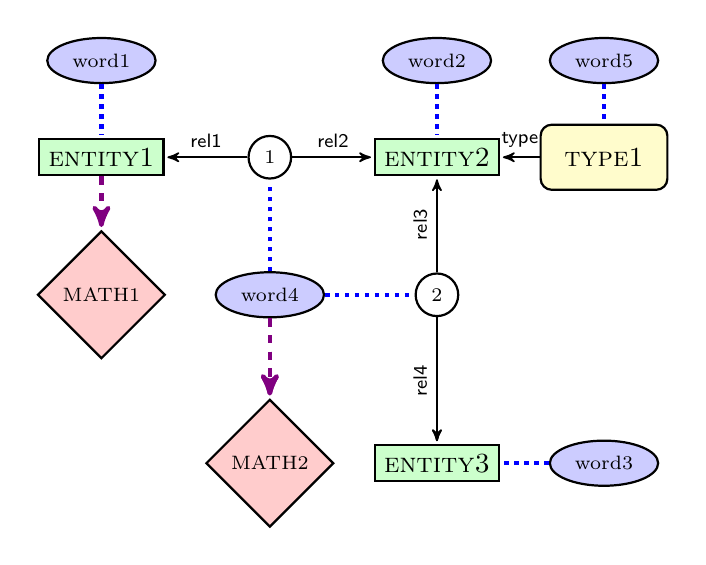
\begin{tikzpicture}[
  font=\sffamily,
  every matrix/.style={ampersand replacement=\&,column sep=0.5cm,row sep=0.5cm,font=\scriptsize},
  entity/.style={draw,thick,rectangle,fill=green!20,font=\sc},
  word/.style={draw,thick,ellipse,fill=blue!20},
  emptyNode/.style={},
  mediator/.style={draw,thick,circle},
  mediatorC/.style={draw,thick,circle,fill=cyan!20},
  mediatorV/.style={draw,thick,circle,fill=violet!20},
  mediatorY/.style={draw,thick,circle,fill=yellow!20},
  entityType/.style={draw,thick,rounded corners,fill=yellow!20,inner sep=.3cm,font=\sc},
  mathType/.style={draw,thick,diamond,fill=red!20},
  mediatorToEntity/.style={->,>=stealth',shorten >=1pt,semithick,black,sloped,above,font=\sffamily\scriptsize},
  typeToEntity/.style={->,>=stealth',shorten >=1pt,semithick,black,sloped,above,font=\sffamily\scriptsize},
  wordToEntity/.style={-,>=stealth',shorten >=1pt,ultra thick,dotted,blue,sloped,above,font=\sffamily\scriptsize},
  entityToMath/.style={->,>=stealth',shorten >=1pt,ultra thick,dashed,violet,sloped,above,font=\sffamily\scriptsize},
  every node/.style={align=center}]

  
  % Edinburgh is the capital of Scotland 
  
  % Position the nodes using a matrix layout
  \matrix{
  \node[word] (w1) {word1}; \& \& \node[word] (w2) {word2}; \&  \node[word] (w5) {word5}; \\ 
  \node[entity] (e1) {entity1}; \& \node[mediator] (m1) {1}; \& \node[entity] (e2) {entity2}; \&  \node[entityType] (t1) {type1}; \\
  \node[mathType] (m3) {MATH1}; \& \node[word] (w4) {word4}; \& \node[mediator] (m2) {2};   \\ 
   \& \node[mathType] (m4) {MATH2}; \& \node[entity] (e3) {entity3}; \&  \node[word] (w3) {word3}; \\
  };
 
 % words to entities
  \draw [wordToEntity] (w1) edge node {}  (e1);
  \draw [wordToEntity] (w2) edge node {}  (e2);
  \draw [wordToEntity] (w3) edge node {}  (e3);
  \draw [wordToEntity] (w5) edge node {}  (t1);
  
  \draw [wordToEntity] (w4) edge node {}  (m1);
  \draw [wordToEntity] (w4) edge node {}  (m2);
  
  
  \draw [entityToMath] (e1) edge node {}  (m3);
  \draw [entityToMath] (w4) edge node {}  (m4);
  
  \draw [entityToMath] (w4) edge node {}  (m4);
 
  \draw [mediatorToEntity] (m1) edge node {rel1}  (e1); 
  \draw [mediatorToEntity] (m1) edge node {rel2}  (e2); 
  
  \draw [mediatorToEntity] (m2) edge node {rel3}  (e2);
  \draw [mediatorToEntity] (m2)[rotate=180] edge node {rel4}  (e3); 
  
  \draw [mediatorToEntity] (t1) edge node {type}  (e2);
  \draw [mediatorToEntity] (m2) edge node {}  (e3);
 
 
\end{tikzpicture} 
\end{center}

% \end{landscape}

% \begin{tikzpicture}
% \node (One) at (-3,0) [shape=circle,draw] {$One$}; 
% \node (Two) at (3,0) [shape=circle,draw] {$Two$};
% \def\myshift#1{\raisebox{-2.5ex}}
% \draw [->,thick,postaction={decorate,decoration={text along path,text align=center,text={|\sffamily\myshift|Some more bent text}}}] (One) to [bend right=45]  (Two);
% \def\myshift#1{\raisebox{1ex}}
% \draw [->,thick,postaction={decorate,decoration={text along path,text align=center,text={|\sffamily\myshift|Some bent text}}}]      (One) to [bend left=45] (Two);
% \end{tikzpicture}


\end{document}

